\documentclass[../competing_bandits.tex]{subfiles}
\begin{document}

\section{Introduction}\label{section:1}

Many modern online platforms simultaneously compete for users as well as learn from the users they manage to attract. This creates a tradeoff between \textit{exploration} and \textit{competition}: firms experiment with potentially sub-optimal options for the sake of gaining information to make better decisions tomorrow, while they need to incentivize consumers to select them over their competitors today. For instance, Google Search and Bing compete for users in the search engine market yet at the same time need to experiment with their search and ranking algorithms to learn what works best.

Platforms routinely deploy A/B tests, and are increasingly adopting  more sophisticated exploration methodologies based on \emph{multi-armed bandits}, a well-known framework for exploration and making decisions under uncertainty. While deploying ``better" learning algorithms for exploration would improve performance, this is not necessarily beneficial under competition, even putting aside the deployment/maintenance costs. In particular, excessive experimentation may hurt platform's reputation and decrease market share in the near term. This would leave the learning algorithms with less users to learn from, which may further degrade platform's performance relative to competitors who keep learning and improving from \emph{their} users, and so forth.

We ask whether competition incentivizes adoption of "better" algorithms for exploration. We investigate this issue via extensive numerical experiments in a stylized duopoly model. In our model, two firms compete for users, and simultaneously learn from them. Each firm commits to a multi-armed bandit algorithm, and \emph{explores} according to this algorithm. Users select between the two firms based on the current reputation score: rewards from the firm's algorithm, averaged over a recent time window. Each firm's objective is to maximize its market share ---the fraction of users coming to them.

\tikzstyle{level 1}=[level distance=3.5cm, sibling distance=4.0cm]
\tikzstyle{level 2}=[level distance=3.5cm, sibling distance=2cm]
\tikzstyle{below} = [align=center]

\begin{figure}
\begin{center}
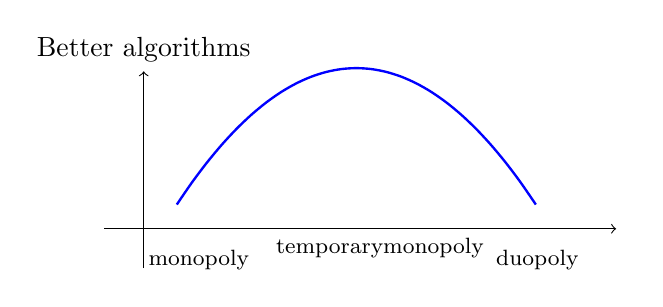
\begin{tikzpicture}
      \draw[->] (-.5,0) -- (6,0) node[right] {};
      \draw[->] (0,-.5) -- (0,2) node[above] {Better algorithms};
      \draw[scale=0.6,domain=0.7:8.3,smooth,variable=\x,blue, line width=0.3mm] plot ({\x},{3.4 - 0.2 * (\x - 4.5)^2});
     \node[below] at (0.7, -0.15) {\footnotesize monopoly};
     \node[below] at (3, 0) {\footnotesize temporary \\ monopoly};
     \node[below] at (5, -0.15) {\footnotesize duopoly};
 \end{tikzpicture}
 \caption{A stylized ``inverted-U relationship" between strength of competition and ``level of innovation".}
\label{fig:inverted-U}
\end{center}
\end{figure}

We consider varying levels of competition, from monopoly to \emph{temporary monopoly} (a duopoly with an early entrant), to a true duopoly in which both firms start at the same time. We find that a ``greedy algorithm" that does not explicitly explore is most beneficial under duopoly. This algorithm also prevails under monopoly, simply because it tends to be easier to deploy. Whereas a temporary monopoly incentivizes more advanced exploration algorithms that perform better in the long run. The disincentives to explore under duopoly arise entirely because of ``reputational costs", rather than R\&D costs (which are absent from our model).

Interpreting the adoption of better algorithms as ``innovation", our findings can be framed in terms of an ``inverted-U relationship" between competition and innovation (see Figure~\ref{fig:inverted-U}). This relationship -- too little or too much competition is bad for innovation, but intermediate levels of competition tend to be better -- is a familiar theme in the economics literature, dating back to \cite{Schumpeter-42}.

Our findings on temporary monopoly shed light on the ``first-mover advantage" phenomenon in the digital economy. In this scenario, the incumbent firm enjoys both a ``data advantage" and a ``reputational advantage". We further investigate which of the two is a stronger barrier to entry. We find that both are strong barriers on its own: removing either one substantially helps the late entrant. Further, the data advantage tends to be a stronger barrier when the incumbent commits to a more advanced bandit algorithm.







\subsubsection{Discussion and related work.}
Our work is related to a longstanding economics literature on competition vs. innovation, \eg \cite{Schumpeter-42,barro2004economic,Aghion-QJE05}. While this literature focuses on R\&D costs of innovation, ``reputational costs" thereof seem new and specific to exploration.

Multi-armed bandits (MAB) is a tractable abstraction for the tradeoff between exploration and \emph{exploitation} (making good near-term decisions based on available information). MAB problems have been studied for many decades, see \cite{Bubeck-survey12} for background. We consider i.i.d. rewards, a well-studied and well-understood MAB model \cite{bandits-ucb1}. We focus on a well-known distinction between the ``greedy" (exploitation-only) algorithm, "naive" MAB  algorithms that separate exploration and exploitation, and better MAB algorithms that combine the two. As a token example of ``near-optimal" bandit algorithms,
we use a classic algorithm called ``Thompson Sampling", see \cite{TS-survey-FTML18} for background.

The study of competition vs. exploration has been initiated in \cite{CompetingBandits-itcs16}. Their model differs from ours in two key respects. First, users do not see any signal about firms' past performance, and instead choose between firms according to the Bayesian-expected reward. Second, they vary the strength of competition using assumptions about (ir)rational consumer behavior, whereas we use early entry. Their results are purely theoretical; their model is amenable to proofs but not to numerical experiments.

The interplay between exploration, exploitation and incentives has been studied in other scenarios: incentivizing exploration in a recommendation system,
    \eg \cite{Kremer-JPE14,Frazier-ec14,Che-13,ICexploration-ec15,Bimpikis-exploration-ms17},
dynamic auctions
    (see \cite{DynAuctions-survey10} for background),
online ad auctions, \eg
    \cite{MechMAB-ec09,DevanurK09,NSV08,Transform-ec10-jacm,Amin-auctions-nips13},
and human computation
    \cite{RepeatedPA-ec14,Ghosh-itcs13,Krause-www13}.
Our setting is also closely related to the "dueling algorithms" framework \cite{DuelingAlgs-stoc11}, but this framework considers offline / full feedback scenarios whereas we focus on online machine learning problems.


\end{document} 